
\chapter{Metody vizualizace a porovnání}

Cílem této knihovny není pouze vizualizovat sekundární strukturu RNA, ale také
usnadnit analýzu rozdílů a podobností mezi více strukturami RNA. Proto jsme se
zaměřili na práci s radiálními diagramy.

Kromě toho jsme rozpoznali potenciál generování distribuce na základě
referenční struktury, jak to dělá nástroj Traveler. Výstupem Traveleru je
soubor ve formátu JSON, který obsahuje informace o vzoru každého nukleotidu a
provedených úpravách.

V důsledku toho jsme se rozhodli používat v našich metodách zmíněné mapování na
referenční strukturu. Náš nástroj je tudíž schopný pracovat s $N$ strukturami,
mezi nimiž je referenční struktura, ze které jsou generovány všechny ostatní
struktury.

\section{Překládání struktur}

Protože jsou struktury odvozené od stejného vzoru jsou typicky velmi podobné,
dává proto smysl mít možnost je přeložit přes sebe, aby splynuli společné části
a vynikly ty rozdílné. Pouhým přeložením podobných struktur přes sebe získámě
poměrně zmatený obrázek, který neukazuje nic zajímavého a není moc přehledný.

\begin{figure}[H]
  \centering
  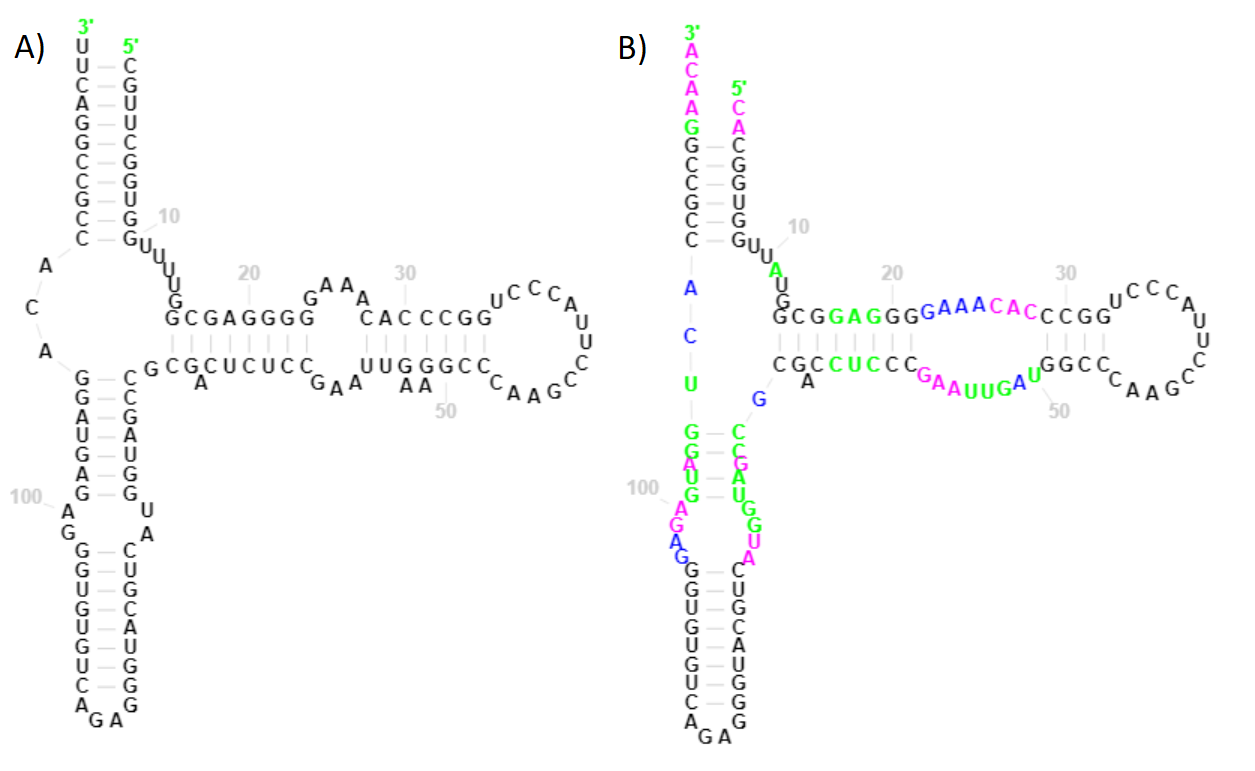
\includegraphics[width=140mm]{../img/kap02/align/structures.png}
  \caption{Struktury vedle sebe.}
\end{figure}

\begin{figure}[H]
  \centering
  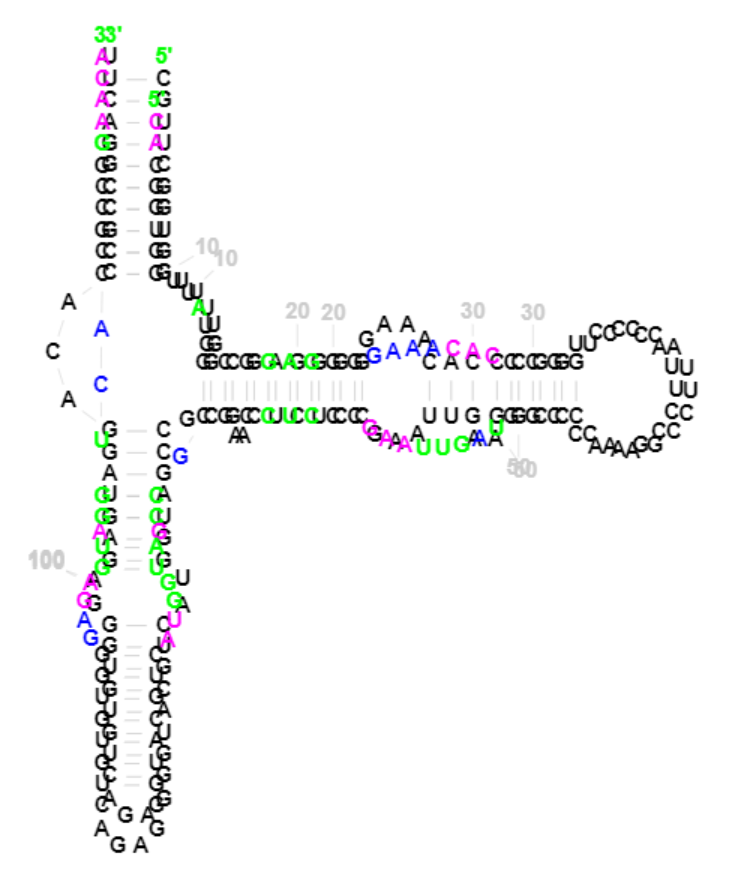
\includegraphics[height=90mm]{../img/kap02/align/unaligned.png}
  \caption{Struktury přeložené přes sebe.}
\end{figure}

Proto bylo důležité přijít s nějakým způsobem pousouvání nebo zarovnání.
Manipulací se strukturou ručně ať už přetažením myši nebo zadáním pozice může
být zbytečně otravné především kvůli přesnému zarovnání, kterého se snažíme
docílit. Přijde nám proto velmi užitečné mít možnost zarovnat sekundární RNA
strukturu na konkrétní nukleotid nebo skupinu nukleotidů ze vzorové struktury.
Tedy pokud je vybraný nukleotid $v$ ze vzorové struktury vzorovým nukleotidem
pro nějaký nukleotid $n$ z ostatních struktur, přesuneme celou strukturu tak,
že se nukleotidy $v$ a $n$ překrývají. 

\begin{figure}[H]
  \centering
  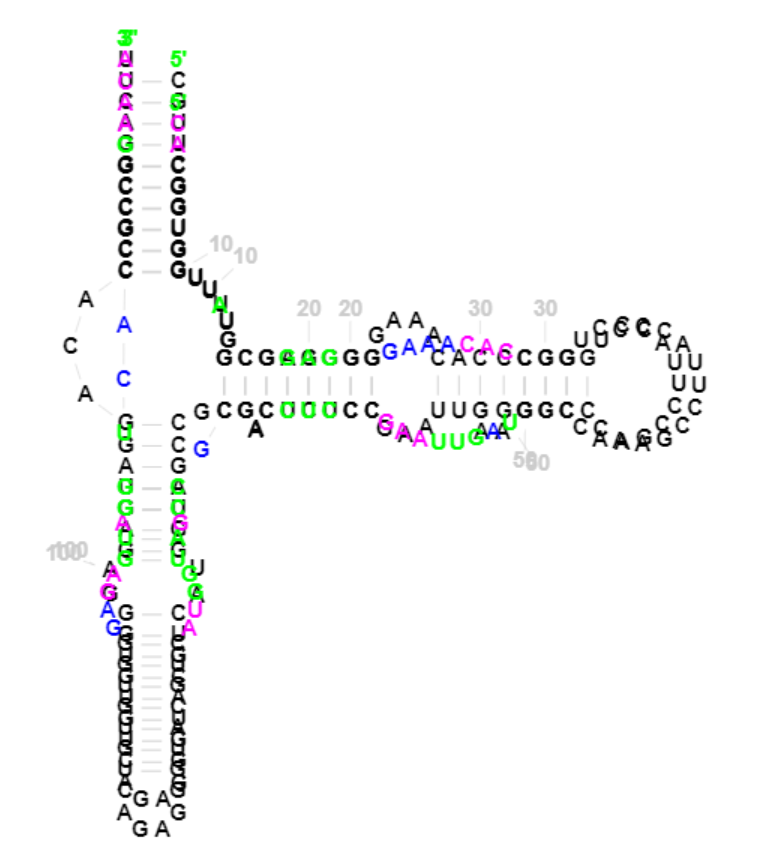
\includegraphics[height=90mm]{../img/kap02/align/alignedAlpha1.png}
  \caption{Struktury přeložené přes sebe a zarovnané.}
\end{figure}

Timto přeložením nemusí být jasné které nukleotidy mají společné a jsou
překryté, a které naopak nejsou společné. Přidáním průhlednosti lze toto
odlišit, protože překryté nukleotidy budou mít sytější barvu oproti těm
nepřekrytým. 

\begin{figure}[H]
  \centering
  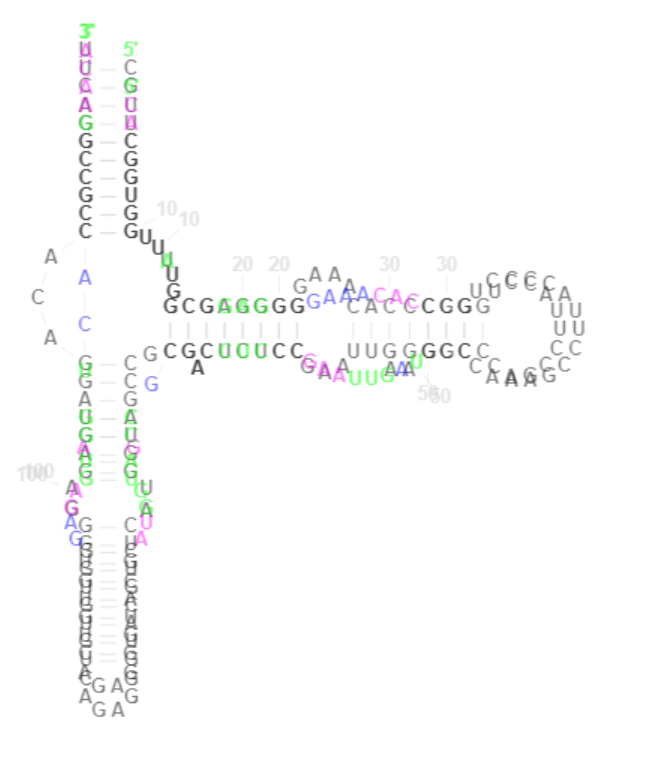
\includegraphics[height=90mm]{../img/kap02/align/aligned.png}
  \caption{Struktury přeložené přes sebe, zarovnané a s průhledností.}
\end{figure}

Zarovnávání struktur bohužel neřeší všechny problémy. Obrázky se můžou zdát
rozmazané, protože ačkoli má nukleotid vzorový nukleotid, od kterého se nijak
neliší může stále jeho pozice být mírně posunutá. Je to dáno metodou generování
dat. Popisky nukleotidů můžou tím pádem vypadat trochu rozmazaně. 

Jako přímočaré řešení by se mohlo zdát posunout jednotilvé nukleotidy, které
jsou blízko, aby dokonale překrývali jejich vzor. Věříme, že by to vyřešilo
zmíněný problém, nicméně naše knihovna tuto funkci nijak přímo neimplementuje.

\section{Transformace na vzor}

Užitečnou metodou je transformace z a na vzorovou strukturu. Každý nukleotid,
který má vzorový nukleotid se přemístí na pozici vzorového nukleotidu a ty
nukleotidy, které vzor nemají jsou schované. Metoda je velmi příjemná pro práci
se dvěmi strukturami, které si jsou podobné nebo pro počáteční přehled co je na
co namapované. Slabá stránka této metody je zjevná při práci s vícero
strukturami nebo strukturami, které jsou velmi odlišné. V takových situacích se
toho na displeji děje hodně a je složité se soustředit a vypozorovat něco
užitečného.

\begin{figure}[H]
  \centering
  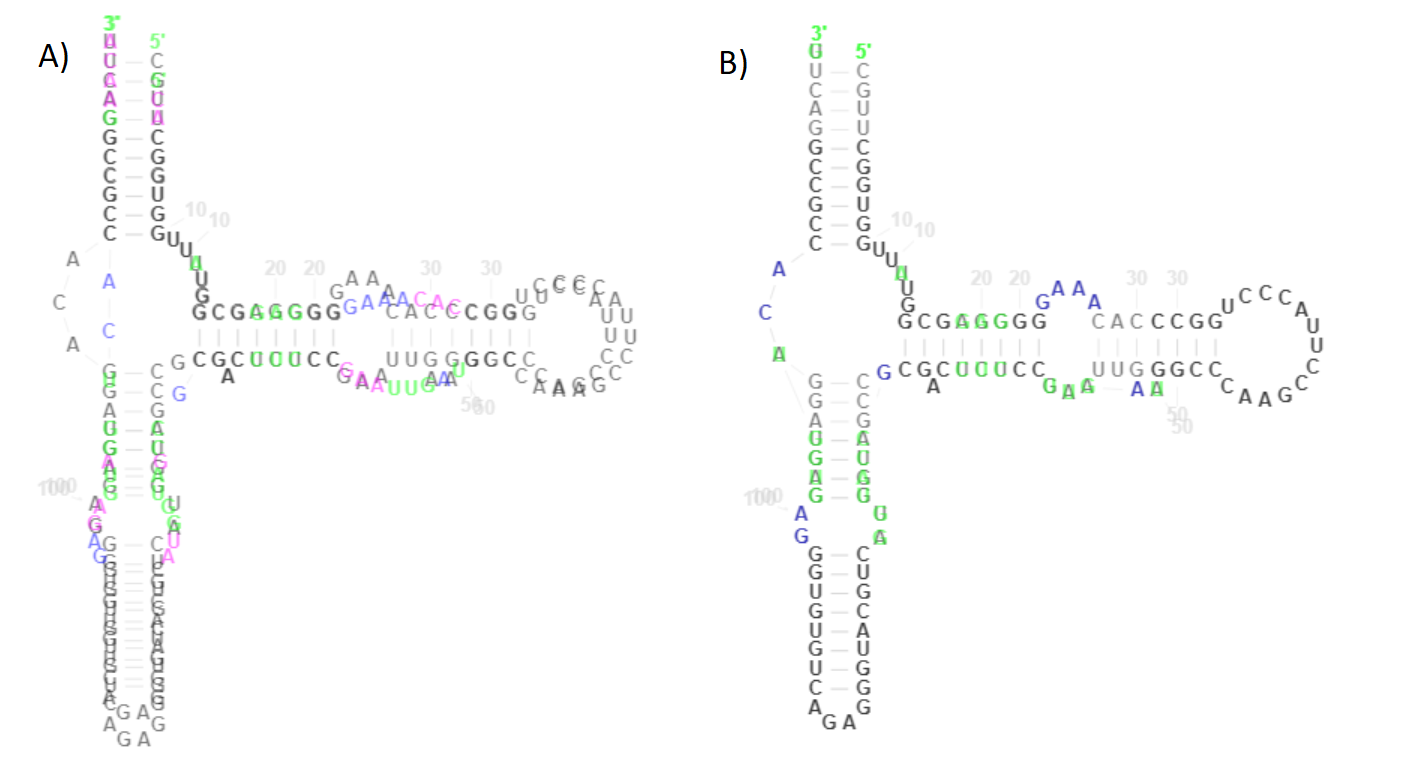
\includegraphics[width=140mm]{../img/kap02/animation.png}
  \caption{Dvě struktury přeložené přes sebe před animací (A) a po animaci (B).}
\end{figure}

\section{Mapovací čáry}

Vědět který nukleotid se na co mapuje může být velmi užitečné pro odhalení
rozdílů a podobností struktur. Snažili jsme se najít další způosob, jak tuto
informaci předat ještě před animací a přišli jsme s čárami, které spojují
nukletid se vzorovým nukleotidem.

\begin{figure}[H]
  \centering
  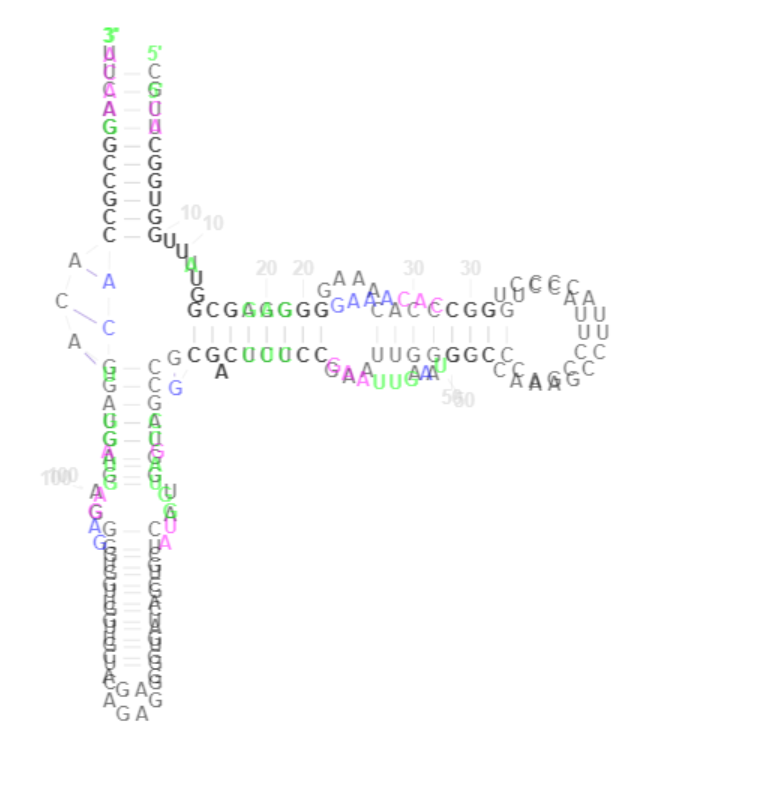
\includegraphics[height=90mm]{../img/kap02/mappingLines/small.png}
  \caption{Dvě struktruy přeložené přes sebe s mapovacíma čárama.}
\end{figure}

Bohužel tento způsob se zvětšující se velikostí struktury stáva velmi
nepřehledným, přesto si myslíme že můžou být užitečné a naše knihovna je
podporuje.

\begin{figure}[H]
  \centering
  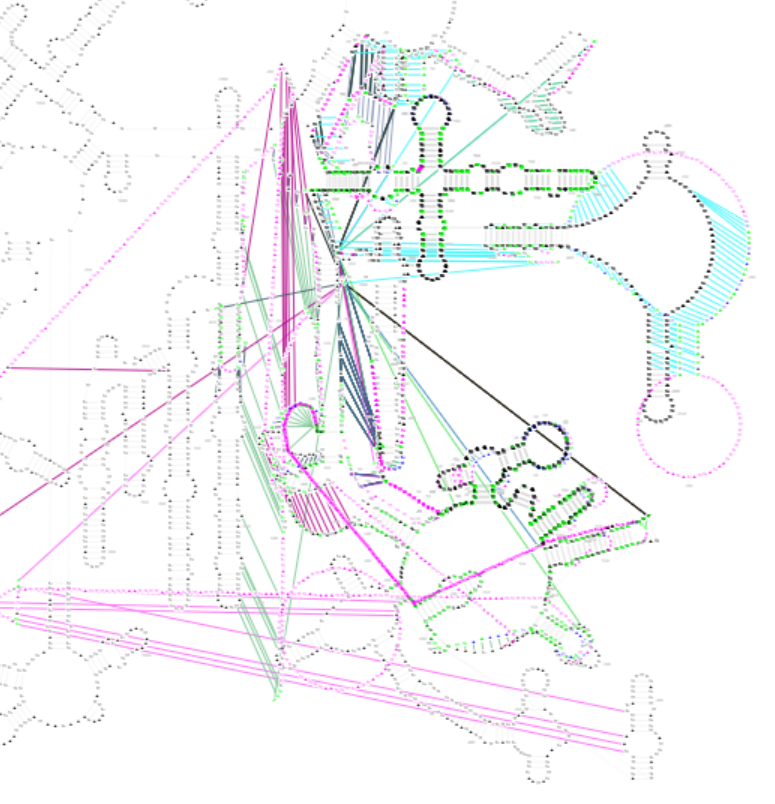
\includegraphics[width=140mm]{../img/kap02/mappingLines/big.png}
  \caption{Výřez z mnoha struktur přeložených přes sebe s mapovacími čárami.
  Každá struktura má vlastní barvu mapovacích čar.}
\end{figure}

\section{Demonstrace metod}

V rámci naší knihovny vznikla i webová
aplikace\footnote{https://michalhercik.github.io/rna-visualizer/}, která
demonstruje možnosti naší knihovny. Umožňuje pracovat vždy jen s jednou metodou
nebo se všemi metodami usnadňující porovnání dvou sekundárních struktur RNA,
které jsou zmíněné v této kapitole.
